%%%%%%%%%%%%%%%%%%%%%%%%%%%%%%%%%%%%%%%%%%%%%%%%%%%%%%%%%%%%%%%%%%%%%%%%%%%
%% ws-procs9x6.tex   :   20-9-2004
%% Text file for Proceedings Trim Size [9in x 6in] written in Latex2E.
%% The content, structure, format and layout of this style file is the 
%% property of World Scientific Publishing Co. Pte. Ltd. 
%% Copyright 1995, 2002 by World Scientific Publishing Co. 
%% All rights are reserved.
%%
%% Proceedings Trim Size: 9in x 6in
%% Text Area: 7.35in (include runningheads) x 4.5in
%% Main Text is 10/13pt					  
%%%%%%%%%%%%%%%%%%%%%%%%%%%%%%%%%%%%%%%%%%%%%%%%%%%%%%%%%%%%%%%%%%%%%%%%%%%

%% Use \tbl{...} command for table caption i.e. to fit table width.
%% Use \caption{...} command for figure caption.
%\documentclass[draft]{ws-procs9x6}  
\documentclass{ws-procs9x6}
\usepackage{pgf}
\usepackage{tikz}


\pgfdeclareimage[width=2cm]{nefroideIdeal}{nefroideIdeal}
\pgfdeclareimage[width=6cm]{nefroideCualquiera}{nefroideCualquiera}
\pgfdeclareimage[width=10cm]{ideaCurvatura}{ideaCurvatura}
\pgfdeclareimage[width=2cm]{nef1}{nef1}
\pgfdeclareimage[width=3cm]{nef2}{nef2}
\pgfdeclareimage[width=3cm]{graf1}{graf1}
\pgfdeclareimage[width=3cm]{graf2}{graf2}
\pgfdeclareimage[width=3cm]{realNefroide}{realNefroide}
\pgfdeclareimage[width=4cm]{realNefroideRotada}{realNefroideRotada}

\pgfdeclareimage[width=4cm]{y-curv}{y-curv}
\pgfdeclareimage[width=4cm]{x-curv}{x-curv}

\pgfdeclareimage[width=4cm]{X-5}{X-5}
\pgfdeclareimage[width=4cm]{Y-5}{Y-5}

\pgfdeclareimage[width=5cm]{primerPiecewise}{primerPiecewise}

\pgfdeclareimage[width=4cm]{nefroideRotada45}{nefroideRotada45}
\pgfdeclareimage[width=5cm]{x-s}{x-s}
\pgfdeclareimage[width=5cm]{y-s}{y-s}
\pgfdeclareimage[width=6cm]{x-s-inter}{x-s-inter}
\pgfdeclareimage[width=15cm]{x-diverse}{x-diverse}



\begin{document}

\title{Curve Detection (we need a better title)\footnote{\uppercase{T}his work is supported by etc, etc.}}

\author{Raquel Pezoa and Luis Salinas\footnote{\uppercase{W}ork partially
supported by grant \ldots}}

\address{Universidad T\'ecnica Federico Santa Mar\'ia, \\
Avenida Espa\~na 1680, \\ 
Valpara\'iso, Chile\\ 
E-mail: rpezoa,lsalinas@usm.cl}

%\author{T.~R. SIMON, S. CLARKE and S.~N. GERALD}

%\address{World Scientific Publishing Co Ltd, \\ 
%57 Shelton Street, \\
%London WC2H 9HE, England\\
%E-mail: wspc@wspc.ox.uk}  

\maketitle

\abstracts{
Ac\'{a} debe ir el abstract.}

\section{Hough Transform}

\subsection{Ellipse}
An ellipse can be described using parametric functions, $x(\theta)$ and
$y(\theta)$.
An ellipse can be drawn using two concentric circles and radial
lines. Let us consider two concentric circles of radii $a$ and $b$ (see Fig. \ref{fig:circles1}), respectively, $a > b$:

\begin{figure}[h!t!pb]
\centering
\begin{tikzpicture}
\draw (-3.0,0) -- (3.0,0); 
\draw (0,-3.0) -- (0,3.0);
\draw (2.0,0) coordinate [label= right:$a$] (a);
\draw (0,1.0) coordinate [label= above:$b$] (b);
 \draw [color=black] circle(2cm);
 \draw [color=black] circle(1cm);
\end{tikzpicture}
\caption{}
\label{fig:circles1}
\end{figure}

The parametric functions that describe the circles are: 
$$x_{a}(\theta) = a \cos\theta \ \ \ y_{a}(\theta)= a \sin\theta$$
$$x_{b}(\theta) = b \cos\theta \ \ \ y_{b}(\theta)= b \sin\theta$$ 

and taking into account that , an ellipse (Fig. \ref{fig:ellipse1})
can be described using two concentric circles, the parametric
functions of the ellipse are:

$$\begin{bmatrix}x(\theta) \\ y(\theta) \end{bmatrix} = \lambda \begin{bmatrix} \cos \rho & \sin \rho \\ -\sin \rho &\cos \rho \end{bmatrix} \begin{bmatrix} a \cos \theta \\ b \sin \theta \end{bmatrix}$$

The ray of the $\theta$ angle (green)

$$x(\theta)= a \cos\theta \ \ \ y(\theta)= b \sin\theta$$

\begin{figure}[h!tpb]
\centering
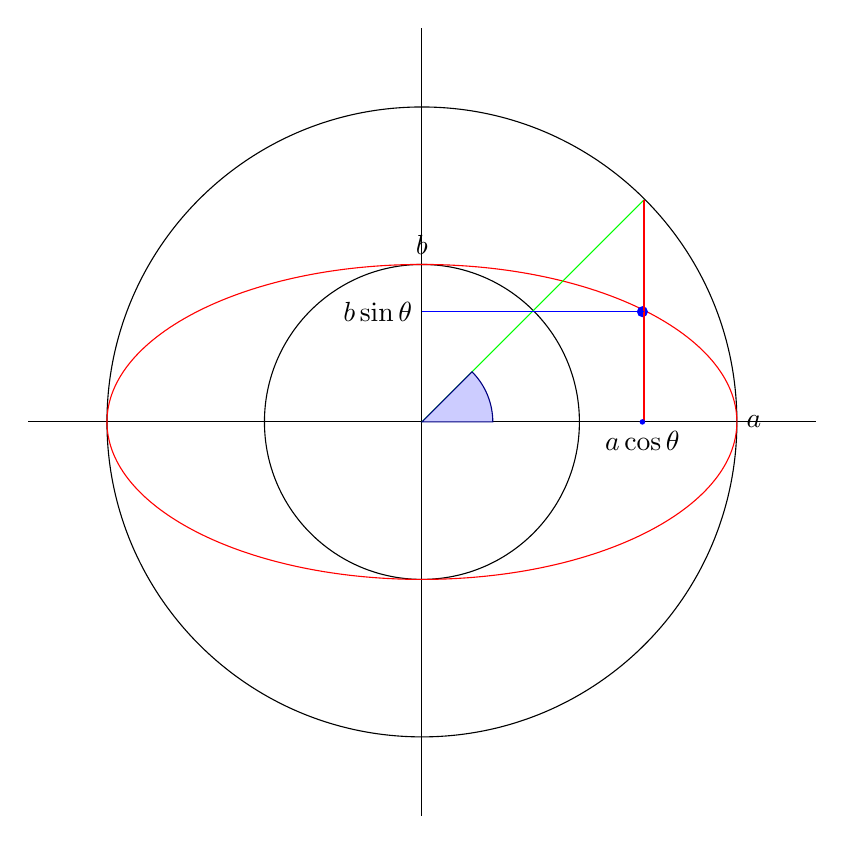
\begin{tikzpicture}
\draw (-5.0,0) -- (5.0,0); 
\draw (0,-5.0) -- (0,5.0);
\draw (4.0,0) coordinate [label= right:$a$] (a);
\draw (0,2.0) coordinate [label= above:$b$] (b);
 \draw [color=black] circle(4cm);
 \draw [color=black] circle(2cm);
\draw [color=red] (0,0) ellipse (4cm and 2cm);

\draw [color=green] (0,0) coordinate (a_1) -- (2.82,2.82) coordinate (a_2);
\fill[blue] (2.8,1.4) circle (2pt);
\draw [color=red] (2.82,2.82) coordinate (a_3) -- (2.82,0) coordinate (a_4);
\coordinate (c) at (intersection of a_1--a_2 and a_3--a_4);
%\fill[blue] (c) circle (2pt);
%\draw [color=blue] (c) -- (0,2.82) coordinate (c_2);
\draw [color=blue] (2.82,1.4) coordinate (c_3) -- (0,1.4) coordinate (c_4);

%\coordinate (d) at (intersection of a_1--a_2 and c_3--c_4);
%\fill[blue] (d) circle (2pt);
\filldraw[fill=blue!20!white, draw=blue!50!black]
(0,0) -- (9mm,0mm) arc (0:45:9mm) -- cycle;

\draw (2.8,0) coordinate [label= below:$a\cos \theta$] (acos);
\fill[blue] (acos) circle (1pt);
\draw (0,1.4) coordinate [label= left:$b\sin \theta$] (asin);
\end{tikzpicture}
\caption{}
\label{fig:ellipse1}
\end{figure}


%%% NEW 
\begin{figure}[h!tpb]
\centering
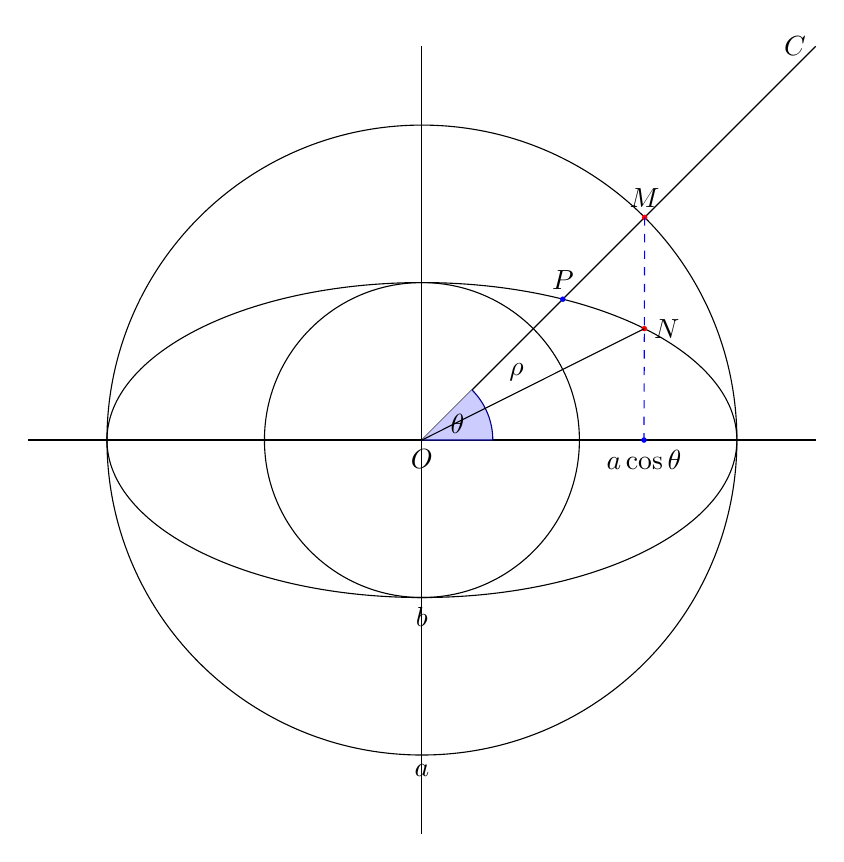
\begin{tikzpicture}
\usetikzlibrary{shapes,snakes}
\usetikzlibrary{calc,intersections,through,backgrounds}

\draw (-5.0,0) -- (5.0,0); 
\draw (0,-5.0) -- (0,5.0);

\coordinate [label=below:$O$] (A) at (0,0);
\coordinate (B) at (2.0,0.0);
\coordinate (B2) at (4.0,0.0);
\coordinate [label=left:$C$] (C) at (5,5);
\coordinate [label=below:$a \cos \theta$] (acos) at (2.82,0);
\coordinate [label=below:$\rho$] (ro) at (1.2,1.1);


\draw (A) -- (B);
\node (D) [name path=D,draw,circle through=(B),label=below:$b$] at (A) {};
\node (E) [name path=E,draw,circle through=(B2),label=below:$a$] at (A) {};
\node (F) [name path=F,draw,ellipse, minimum height=4cm,minimum width=8cm] at (A){};
\draw [name path=A--C] (A) -- (C);


% Name the coordinates, but do not draw anything:
\path [name intersections={of=F and A--C}];
\coordinate [label=above:$P$] (i-1) at (intersection-1);
\fill[blue] (i-1) circle (1pt);

\path [name intersections={of=E and A--C}];
\coordinate [label=above:$M$] (j-1) at (intersection-1);
\fill[red] (j-1) circle (1pt);

\filldraw[fill=blue!20!white, draw=blue!50!black]
(0,0) -- (9mm,0mm) arc (0:45:9mm);
\draw(25:5mm) node {$\theta$};

\draw [name path=M--acos,dashed,blue] (j-1) -- (acos);
\fill[blue] (acos) circle (1pt);

\path [name intersections={of=M--acos and F}];
\coordinate [label=right:$N$] (k-1) at (intersection-1);
\fill[red] (k-1) circle (1pt);

\draw [name path=A--N] (A) -- (k-1);










\end{tikzpicture}
\caption{}
\label{fig:ellipse1}
\end{figure}





, and the radii of the two circles are the lengths of the
semi-minor and semi-major axes.

\section{Generalized Hough Transform}
\label{subsec:prod}
Many shapes are more complex than a line or a circle, and the
Generalized Hough Transform  (GHT) allows to find arbitrary shapes using the
evidence-gathering process of the Hough Transform (HT).

The Generalized Hough Transform was introduced by D. H. Ballard in
\cite{ballard}.
To represent an arbitrary shape, the GHT uses directional information
of the shape. 
Directional information is associated with the edge representation of
the shape. 

To understand the issue of directional information, it will be explain
the approach described by Nixon and Aguado in \cite{nixon}.

A \emph{model shape} can be described as a vectorial function:
$$ \upsilon(\theta) = x(\theta)\begin{bmatrix} 1 \\ 0\end{bmatrix} + y(\theta)\begin{bmatrix} 0\\ 1\end{bmatrix}$$ 

$x(\theta)$ and $y(\theta)$ correspond to parametric functions that
    describes the points of the curve. The model shape is an
    \emph{ideal} curve can be thought as a pattern curve. The
    idea is to match the model shape against a shape in any image.
Therefore, during the matching process, the arbitrary shape could be
rotated, scalated or translated (with respecto to the model shape),
and its representation would be:

$$ \omega(\theta,b,\lambda,\rho)= b + \lambda R(\rho)\upsilon(\theta)$$

 $b=\begin{bmatrix}b_{x} \\ b_{y}\end{bmatrix}$ is the translation
vector, $\lambda$ is the scale factor and $R(\rho)$ corresponds to the
rotation matrix.

Let us consider a curve called \emph{nephroid}, whose parametric equations are:
$$x(\theta)=a(3\cos(\theta) - \cos(3\theta)), \ \ y=a(3\sin(\theta) - sin(3\theta))$$

\begin{figure}
\centering
\pgfuseimage{realNefroide}
\caption{Nephroid.}
\end{figure}

Matlab code for the generation of nephroid:
\begin{verbatim}
t=0:0.01:2*pi;
a=0.4;
x=a*(3*cos(t)-cos(3*t));
y=a*(3*sin(t)-sin(3*t));
plot(x,y);
\end{verbatim}

The model shape equation is:
$$ \upsilon(\theta) =  \begin{bmatrix} a(3\cos(\theta) - \cos(3\theta)) \\ a(3\sin(\theta) - sin(3\theta))\end{bmatrix}$$ 

but if the nephroid is rotated, scalated and translated:

$$ \omega(\theta,b,\lambda,\rho) = \begin{bmatrix} 2 \\ 3 \end{bmatrix} + 2 \begin{bmatrix} \cos(\rho) & -\sin(\rho) \\ \sin(\rho) & \cos(\rho) \end{bmatrix} \begin{bmatrix} a(3\cos(\theta) - \cos(3\theta)) \\ a(3\sin(\theta) - sin(3\theta))\end{bmatrix}$$

$\rho=\frac{\pi}{4}$ and $a=0.4$, and the nephroid is shown in
Fig. \ref{fig:nefRot}:

\begin{figure}[h!tpb]
\centering
\pgfuseimage{realNefroideRotada}
\caption{Rotated, scalated and translated nephroid.}
\label{fig:nefRot}
\end{figure}

\newpage

\begin{verbatim}
t=0:0.01:2*pi;
a=0.4;
b=[2;3]
lam=2;
wx= b(1,1) + lam*(cos(pi/4).*x2 - sin(pi/4).*y2);
wy= b(2,1) + lam*(sin(pi/4).*x2 + cos(pi/4).*y2);
plot(wx,wy);
\end{verbatim}

If we know the parametric functions $x(\theta)$ and $y(\theta)$, to
find the model shape in a new image, called $I$, we have to find the
parameters: $b$, $\lambda$ and $\rho$. 
But we do not know, $x(\theta)$ and $y(\theta)$, thus, the problem is
complex.

If it is considered that the model shape will not be rotated nor
scaleted, only translated, we should look for the parameter $b$, which
is defined as:

\begin{equation}
b=\omega(\theta,b,\lambda,\rho)-\lambda R(\rho)\upsilon(\theta)
\label{eq:5-73}
\end{equation}

$\omega(\theta)$ and $\upsilon(\theta)$ are not known, there are only
points of the shape in image $I$. The points in the image $I$ will be
called $\omega_{i}=(\omega_{xi},\omega_{yi})$,

$$ b=\omega_{i}-\lambda R(\rho)\upsilon(\theta)$$ 
and it is obtained a system with four unknowns and with as many
equations as points in the image. 

%Using the evidence gathering approach of the Hough Transform, a
%four-dimensional accumulator space should be used. For each potential
%value of $b$, $\lambda$ and $\rho$ it will be traced a \emph{point
%  spread function} by considering all the values of $\theta$.

The GHT add informations gradient direction information in order to
use the gather evidence process of the HT.  
To use Eq. \ref{eq:5-73} it is necessary to know the model shape
$\upsilon(\theta)$ and the shape $\omega(\theta)$, but only the points
$w_{i}$ are known.

To define the gradient direction at a point in the arbitrary model:

\begin{equation} 
\begin{array}{cc}
\phi\sp{\prime}(\theta) =
\frac{y\sp{\prime}(\theta)}{x\sp{\prime}(\theta)}
& \text{ and }\hat{\phi\sp{\prime}}(\theta)=\tan^{-1}(\phi\sp{\prime}(\theta))
\end{array}
\label{eq:5-75}
\end{equation}


Finally the arbitrary shape is represented by a table, which is called
the R-table.

The R-table has the following form:



\begin{table}[ph]
\tbl{R-table.}
{\footnotesize
\begin{tabular}{cc}
\hline
$\hat{\phi}\sp{\prime}_{i}$ & $\gamma=(r,\alpha)$ \\\hline
0 & $(r_{0},\alpha_{0})$,$(r_{1},\alpha_{1})$,$(r_{2},\alpha_{2})$  \\
$\Delta \phi$ & $(r_{0},\alpha_{0})$,$(r_{1},\alpha_{1})$,$(r_{2},\alpha_{2})$  \\
\hline
\end{tabular}\label{tab:r-table} }
\vspace*{-13pt}
\end{table}


\subsection{The Problem}


The idea is to match a \emph{model shape} (``ideal world'') against a
shape in any image.  
However, the shape in the image has a different location, orientation
and scale, see Fig. \ref{fig:1}.

\begin{figure}
\centering
\pgfuseimage{nefroideIdeal}
\caption{Model shape.}
\label{fig:1}
\end{figure}

\begin{figure}
\centering
\pgfuseimage{nefroideCualquiera}
\caption{Shape in an image.}
\label{fig:2}
\end{figure}


\subsection{Goal of the Study}
The goal of this study is to describe a model shape (``ideal world'')
of a digital image in function of its arc length ($s$) and curvature
($\kappa$), which will be used in the Generalized Hough Transform.
The hipothesis is that this description will be a better alternative
instead of the R-Table used in the Generalized Hough Transform. 
This means to replace the $\hat{\phi}\sp{\prime}_{i}$ of the R-table
by the arc length ($s$) and to replace the $\gamma=(r,\alpha)$ by the
curvature ($\kappa$) of the model shape.

\section{Theoretical Framework}
\subsection{Explanation of use of Arc Length and Curvature}
Let r(t) be the curve describe by:
$$r(t)=\begin{bmatrix} x(t)  \\ y(t)\end{bmatrix} = \begin{bmatrix}(1 - a\cos(2t))\cos(t) \\ (1 - a\cos(2t))\sin(t)\end{bmatrix}, \ \ a=0.45 $$

\begin{figure}[h!tpb]
\centering
\pgfuseimage{nef1}
\caption{$r(t)$.}
\end{figure}


\begin{figure}[h!tpb]
\centering
\pgfuseimage{nef2}
\caption{Rotated $r(t)$.}
\end{figure}


\begin{figure}[h!tpb]
\centering
\pgfuseimage{graf1}
\caption{Curvature $\kappa$ of $r(t)$}
\end{figure}


\begin{figure}[h!tpb]
\centering
\pgfuseimage{graf2}
\caption{Curvature $\kappa$ of rotated $r(t)$}
\end{figure}


\newpage
\subsection{Arc Length}
\label{sec:arclength}
It is necessary to get the arc length of the arbitrary
shape. The algorithm called \emph{getArcLength} was used.

\subsection{Curvature}
%Intuitively, the curvature is the rate of change in edge direction.

The curvature is normally defined considering a parametric form of a curve.
The points of the curve of a digital image can be characterized  as:
    $$r(t)=\begin{bmatrix}x(t) \\ y(t) \end{bmatrix}$$
    
where $t$ defines an arbitrary parameter, but we could think that the
trace of the curve is the motion of a point and $t$ is related with
time. Changes in the position vector are given by the tangent vector
function of the curve $r(t)$:

    \begin{equation}
      \dot{r}(t)=\begin{bmatrix}\dot{x}(t) \\ \dot{y}(t) \end{bmatrix} \ \ \rightarrow \text{{\color{blue} Velocity}}
    \end{equation}

%The magnitud of the velocity is: $\lvert \dot{r(t)} \rvert =\sqrt{\dot{x}^{2}(t) + \dot{y}^{2}(t)}$. 
%The direction of the velocity is: $\rho(t)=\tan^{-1}\frac{\dot{y}(t)}{\dot{x}(t)}$

The curvature at a point $r(t)$ describes the change in the direction $\rho(t)$ with respect to the changes in the arc lenght:
$$\kappa(t)=\frac{d\rho(t)}{ds}$$
where $\rho$ is the angle of the tangent to the curve.

We can obtain that:
    $$\kappa(t) = \frac{\dot{x}(t)\ddot{y}(t)- \dot{y}(t)\ddot{x}(t)}{[\ddot{x}^{2}(t) + \ddot{y}^{2}(t)]^{\frac{3}{2}}}$$


but we do not have the parametric form of the curve! In a digital
image we only have the ``points of the curve'', so we need to find a
good way to calculate the curvature.

\section{Getting the Curvature}


\subsection{Measurement of Edge Direction}
Intuitively, the curvature is the rate of change in edge direction,
thus, a way to compute curvature in digital images is to measure the
change of edge direction.



Fig. \ref{fig:curvIdea} shows an arbitrary curve and three points:
$t_{k-1}=r(s_{k-1})$, $t_{k}=r(s_{k}), t_{k+1}=r(s_{k+1})$.
$r(s_{k})$ corresponds to the point of the curve which is described as
a function of the arc length $s$. $T(s_{k})$ is the tangent vector at
point $t_{k}$.

\begin{figure}[h!tpb]
\centering
\pgfuseimage{ideaCurvatura}
\caption{Curvature in an arbitrary curve.}
\label{fig:curvIdea}
\end{figure}


The change of in edge direction is given by:
\begin{equation}
\frac{\lVert T(s_{k})-T(s_{k-1})\rVert}{\Delta s}  \approx \kappa(s_{k})
\label{eq:one}
\end{equation}
and the tangent vector $T(s_{k})$ is:
$$T(s_{k})=r(s_{k+1}) - r(s_{k}), \ \ T(s_{k-1})=r(s_{k}) - r(s_{k-1})$$

the numerator of fraction of Eq. \ref{eq:one} is given by:
$$\lVert T(s_{k}) - T(s_{k-1}) \rVert = \lVert r(s_{k+1})  - 2 r(s_{k}) + r(s_{k-1}) \rVert$$

$r(s_{k})$ is a point in the digital image, which finaly is
represented as the coordinates of the point in the image, thus,
$r(s_{k}) = \begin{bmatrix}x_{k} \\  y_{k} \end{bmatrix}$ and the curvature would be:

\begin{equation}
\kappa(s_{k}) \approx \sqrt{(x_{k+1} -2 x_{k} + x_{k-1})^{2} + (y_{k+1} -2 y_{k} + y_{k-1})^{2}}
\label{eq:two}
\end{equation}


\subsection{Measurement of Angular Change}
$\ldots$

\subsection{Experimental Results}
Since the the measurment of change of edge direction and angular
change was developed using discrete points, the obtained results were
very ragged.
For this reason, the use of the discrete points of the images are not
appropiate to get a good curvature.

The best way to get the curvature is using the equation $\kappa(s) =
\lVert r\sp{\prime\prime}(s) \rVert$, for which is necessary to have
an equation of the model shape.
To get the equation, splines will be used.


\section{Splines}
Spline is a piecewise polynomial function that can have locally very
simple form.  
A cubic spline is a spline constructed of piecewise third-order
polynomials which has the following form:

Given n data points $(x_{1},y_{1}) \ldots (x_n,y_n)$\\
$S_{1}(x) = y_{1} + b_{1}(x-x_{1}) + c_{1}(x-x_{1})^{2} + d_{1}(x-x_{1})^{3} \ \ for x \in [x_{1},x_{2}]$\\
$S_{2}(x) = y_{2} + b_{2}(x-x_{2}) + c_{2}(x-x_{2})^{2} + d_{1}(x-x_{2})^{3} \ \ for x \in [x_{2},x_{3}]$\\
$\vdots$\\
$S_{n-1}(x) = y_{n-1} + b_{n-1}(x-x_{n-1}) + c_{n-1}(x-x_{n-1})^{2} + d_{n-1}(x-x_{n-1})^{3} \ \ for x \in [x_{n-1},x_{n}]$

The ${\color{blue}3(n-1)}$ unknowns $(b's, c's, d's)$ are choosen to satisfy the
following constraints:

\begin{enumerate}
\item \textbf{Interpolation Condition}: $S_{i}(x_{i})=y_{i}$ for $i=1
  \ldots n-1$ and to have continuity on the overall function:

$$S_{i}(x_{i+1})=S_{i+1}(x_{i+1})=y_{i+1}$$

And for the last value of $x$, $S_{n-1}(x_{n})=y_{n}$

\item \textbf{Smoothness Condition 1}: At the interior points:

$$S_{i}\sp{\prime}(x_{i+1})=S_{i+1}'(x_{i+1})$$

\item \textbf{Interpolation Condition}: At the interior points:
$$S_{i}''(x_{i+1})=S_{i+1}''(x_{i+1})$$

\end{enumerate}

Next section describes the use of cubic spline for getting an analytic
description of an arbitrary curve.

\subsection{Implementation of Cubic Splines}
We want to find the cubic spline that interpolate the following curve:
\begin{figure}
\centering
\pgfuseimage{nefroideRotada45}
\end{figure}

We do not have tha analytic equation of the curve, thus, we need to
interpolate using the data $(x,y)$, which correspond to the
coordinates of each pixel of the image.

We also have the arc length (using \emph{getArcLength},
Sec. \ref{sec:arclength}), $s$, of the curve, thus we have the values
of coordinate $x$ and $y$ in function of $s$:

\begin{center}
\begin{tabular}{c c c }\\\hline
$s$ &$x(s)$ & $y(s)$  \\\hline
0 &31 &259  \\\hline
1,4142 &32 &258  \\\hline
2,4142 & 32 &257  \\\hline
\vdots &\vdots &\vdots \\\hline
1.438 &31 & 261 \\\hline
\end{tabular}
\end{center}

Fig. \ref{fig:x-s} and \ref{} show $x(s)$ and $y(s)$, respectively.

\begin{figure}
\centering
\pgfuseimage{x-s}
\label{fig:x-s}
\end{figure}

\begin{figure}
\centering
\pgfuseimage{y-s}
\label{fig:y-s}
\end{figure}

To interpolate $x(s)$ we build 248 intervals $[s_{i},s_{i+1}], s \in
[0,curveLength]$, and they were of the form:
$$[0,4.4142], [4.4142, 9.8284], [9.8284, 14.8284] \dots [1437,1438]$$

Thus, a spline of  247 picewise polynomials were obtained. The generateSpline\_v2 function was used:

\begin{verbatim}
function generateSpline_v2(alTable,nameIm)
x_curv=alTable(:,1);
y_curv=alTable(:,2);
arcCoord = alTable(:,3);
N=5;

%%%generation of intervals
absisa5=generaCadaNpuntos(arcCoord',N);
X_5=generaCadaNpuntos(x_curv',N);
size(X_5)
Y_5=generaCadaNpuntos(y_curv',N);

%%%generation of spline
pp=spline(absisa5,X_5);
\end{verbatim}

The Matlab function $spline(x,Y)$ returns the $pp$ structure, wich have the following form:
\begin{verbatim}
pp = 

      form: 'pp'
    breaks: [1x248 double]
     coefs: [247x4 double]
    pieces: 247
     order: 4
       dim: 1
\end{verbatim}

where $pp.coefs$ contains the four coefficients of the 247 piecewise
polynomials.  
For instance, considering a polynomial $S_{i}(s)= c_{0} +
c_{1}(s-s_{i})+c_{2}(s-s{i})^{2}+c_{3}(s-s_{i})^{3}$, the three first piecewise polynomials
have the following coefficients:

\begin{table}[h!tpb]
\centering
\begin{tabular}{c  c  c  c  c  c}\\\hline
$c_{3}$ & $c_{2}$ & $c_{1}$ &$c_{0}$ &$absisa5$ & polynomial\\\hline
-0.0020 & 0.0244 & 0.1579 & 31 & 0 &  $31 +0.1579(s-s_{i})+0.0244(s-s{i})^{2}-0.0020(s-s_{i})^{3}$\\\hline
-0.0020 & 0.0022 & 0.2559 & 32 & 4.4142 &$31 +0.2559(s-s_{i})+0.0022(s-s{i})^{2}-0.0020(s-s_{i})^{3}$\\\hline
0.0048 & -0.0350 & 0.0544 & 31 & 9.8284 &$31 +0.0544(s-s_{i})-0.0350(s-s{i})^{2}-0.0048(s-s_{i})^{3}$\\\hline
\end{tabular}\\

\label{tab:coef}
\caption{Three first the piecewise polynomials of the spline.}
\end{table}

The plot of the the interpolation of $x(s)$ is:

\begin{figure}
\pgfuseimage{x-s-inter}
\end{figure}

\begin{figure}
\centering
\pgfuseimage{x-diverse}
\end{figure}





Now we have polynomials to represent $x(s)$, therefore, we can
calculate $x\sp{\prime}(s)$ and $x\sp{\prime\prime}(s)$.  We are
interested in $x\sp{\prime\prime}(s)$ (for the calculation of the
curvature $\kappa$), which can be obtained as follows:


$$x(s)= c_{0} + c_{1}x+c_{2}x^{2}+c_{3}x^{3}$$
$$x\sp{\prime\prime}(s) =  2c_{2}+ 6c_{3}x^{3}$$


Considering the example of Tab. \ref{tab:coef}, the coefficients of
the first three polynomials of $x\sp{\prime\prime}(s)$ (that
correspond to lines) are:

\begin{table}[h!tpb]
\centering
\begin{tabular}{|c | c | c | c |}\\\hline
$6c_{3}$ & $2c_{2}$  \\\hline
-0.0121 & 0.0489  \\\hline
-0.0121 & 0.0045  \\\hline
0.0289 & -0.0699  \\\hline
\end{tabular}\\

\label{tab:coef2}
\caption{Three first coefficients of the piecewise polynomials of
  $x\sp{\prime\prime}(s)$.}
\end{table}

The plot of  $x\sp{\prime\prime}(s)$ is shown in Fig. \ref{fig:xprimeprime}

\begin{figure}[h!tpb]
  \centering
%  \pgfuseimage{}
%  \caption{}
%  \label{fig:y5}

\end{figure}

\subsection{B-splines}
Least-square spline approximation was used. 
The Matlab function \emph{spap2(knots,k,x,y)} was used, which returns the B-form of the spline of order $k$:
\begin{itemize}
\item $knots$: sequence of knots.
\item $k$: order of spline.
\item $x$: abscisas
\item $y$: ordenadas
\end{itemize}

\emph{augknt(knots,k)} returns a nondecreasing and augmented knot sequence that has the first and last knot with exact multiplicity $k$. 

\begin{verbatim}
[alTable,M,Angulos,magx,magy,imgris,newIm]=generaGrafico_v3('nefroideRotada45.png');
misX=[alTable(:,3)];
misX=misX';
mis_knots= augknt(misX,1);
spap2(mis_knots,4,alTable(:,3),alTable(:,1));
sp0=spap2(mis_knots,4,alTable(:,3),alTable(:,1));
sp0=spap2(mis_knots,4,alTable(:,3),alTable(:,1))
\end{verbatim}

\begin{verbatim}
function [pp,A,B,alTable,x_curv,y_curv,X_5,absisa5,x,y] = generateSpline(alTable,nameIm)
x_curv=alTable(:,2);
y_curv=alTable(:,1);
arcCoord = alTable(:,3);
N=5;
absisa5=generaCadaNpuntos(arcCoord',N);
X_5=generaCadaNpuntos(x_curv',N);
Y_5=generaCadaNpuntos(y_curv',N);
\end{verbatim}



\newpage

\section*{Acknowledgments}
This is where one acknowledge funding bodies etc.  Note that section
numbers are not required for Acknowledgments, Appendix or References.





\begin{thebibliography}{0}
\bibitem{ja} M. Barranco and J. R. Buchler, {\it Phys. Rev.}
{\bf C34}, 1729 (1980).

\bibitem{ballard} D. H. Ballard, Generalizing the Hough Transform to
  detect Arbitrary Shapes. (1979).

\bibitem{nixon} M. Nixon and A. Aguado. Feature Extraction and Image
  Processing.

\end{thebibliography}

\end{document}
